\documentclass[aspectratio=169,xcolor={usenames,dvipsnames,svgnames,table},10pt,usepdftitle=false,hyperref={bookmarksdepth=3}]{beamer}

\usetheme[titleformat frame=smallcaps, numbering=fraction]{metropolis}
\usefonttheme{professionalfonts}
%\setbeamertemplate{frame footer}{\insertshorttitle\quad---\quad\insertshortauthor}

\usepackage{polyglossia}
\setmainlanguage{english}
\setotherlanguage{german}

\usepackage{appendixnumberbeamer} % Don't count appendix, references etc. in slide count
\usepackage{amsmath,amssymb,amsfonts}
\usepackage{graphicx}
\usepackage{perpage}
\usepackage{enumitem}
\usepackage[absolute,overlay]{textpos}
\usepackage{multirow, booktabs, tablefootnote, wrapfig}

\usepackage{booktabs} % for toprule
\usepackage{tabularx} % alternative tabular environment
\newcolumntype{R}{>{\raggedleft\arraybackslash}X} % custom tabular option

\MakePerPage{footnote}
%\usepackage{graphicscache} % automatic image size reduction (comment out, if not required)
%\usepackage{multimedia} % For video playback using viewer-internal player

\usepackage[style=numeric,natbib]{biblatex}
\addbibresource{literature.bib}
\renewcommand*{\bibfont}{\normalfont\footnotesize}
%\renewcommand{\labelitemi}{\(\fsbullet\)}

\usepackage{caption}
\captionsetup[figure]{font={small}}

\usepackage{bookmark}
\makeatletter
\apptocmd{\beamer@@frametitle}{\only<1>{\bookmark[page=\the\c@page,level=3]{#1}}}%
{\message{** patching of \string\beamer@@frametitle succeeded **}}%
{\message{** patching of \string\beamer@@frametitle failed **}}%
\makeatother



% No space around figures
\makeatletter
\renewenvironment{figure}[1][]{%
  \def\@captype{figure}%
  \par\centering}
  {\par}
\makeatother

%%%%%%%%%%%%%%%%%%%%%%%%%%%%%%%%%%%%%%%%%%%%%%%%%%%%%%%%%%%%%%%%%%%%%%%%%%%%%%%%

\hypersetup{pdftitle=Presentation}
\title{Citi-Bike Data Challenge}
\author[Jonathan Lennartz]{Jonathan Lennartz}
\institute[University of Bonn]{

\begin{textblock*}{8cm}(7cm,6cm) % {block width} (coords)

    \vspace*{0.1cm}
    \begin{figure}[b]
        %\centering
        \hfill
        
\includegraphics[width=0.3\textwidth]{../assets/axa_logo.png}
    \end{figure}

\end{textblock*}}

\begin{document}

\maketitle

%%%%%%%%%%%%%%%%%%%%%%%%%%%%%%%%%%%%%%%%%%%%%%%%%%%%%%%%%%%%%%%%%%%%%%%%%%%%%%%%
% Slide 1: Is there an opportunity?
%%%%%%%%%%%%%%%%%%%%%%%%%%%%%%%%%%%%%%%%%%%%%%%%%%%%%%%%%%%%%%%%%%%%%%%%%%%%%%%%

\begin{frame}{Is there an opportunity?}
    \begin{itemize}
        \vspace{0.3cm}
        \item \textbf{If we reduce claims we}
        \begin{itemize}
            \item [1.] reduce temporary cost coverage, legal fees, administrative costs, etc and
            \item [2.] get publicity and improve brand reputation
        \end{itemize}
        
        \vspace{0.3cm}

        \item \textbf{Scale of the problem:}
        \begin{itemize}
            \item[-] Roughly 5,000 crashes involving bikes and cars annually
            \item[-] \~40\% of these are likely Citi Bike users
            \item $\rightarrow$ \textbf{\~2000 cases per year}
        \end{itemize}
    \end{itemize}
\end{frame}

%%%%%%%%%%%%%%%%%%%%%%%%%%%%%%%%%%%%%%%%%%%%%%%%%%%%%%%%%%%%%%%%%%%%%%%%%%%%%%%%
% Slide 2: How can we do something?
%%%%%%%%%%%%%%%%%%%%%%%%%%%%%%%%%%%%%%%%%%%%%%%%%%%%%%%%%%%%%%%%%%%%%%%%%%%%%%%%

\begin{frame}{How can we do something?}
    \begin{columns}
        \begin{column}{0.5\textwidth}
            \textbf{Nudging is promising:}
            
            \begin{itemize}
                \item[-] \textbf{Effective}: Up to 30\% crash reduction demonstrated
                \item[-] \textbf{Versatile} delivery channels:
                \begin{itemize}
                    \item Within Citi Bike app
                    \item AXA mobile app
                    \item 3rd party wearables
                \end{itemize}
                \item[-] \textbf{Multiple intervention types:}
                \begin{itemize}
                    \item Push notifications
                    \item Incentive programs
                    \item Route suggestions
                \end{itemize}
            \end{itemize}
        \end{column}
        
        \begin{column}{0.5\textwidth}
            \textbf{Key considerations:}
            \begin{itemize}
                \item \textcolor{orange}{\textbf{Nudging fatigue:}} Keep interventions rare to maintain effectiveness
                \item \textcolor{orange}{\textbf{Neighborhood discrimination:}} Avoid reinforcing existing spatial inequalities
                \item \textcolor{orange}{\textbf{Usage disincentive:}} Don't discourage overall bike usage
            \end{itemize}
            
            \vspace{0.3cm}
            
            \textbf{Solution:} Precise identification of dangerous \textit{area × time} combinations
        \end{column}
    \end{columns}
\end{frame}

%%%%%%%%%%%%%%%%%%%%%%%%%%%%%%%%%%%%%%%%%%%%%%%%%%%%%%%%%%%%%%%%%%%%%%%%%%%%%%%%
% Slide 3: Why hasn't this been done before?
%%%%%%%%%%%%%%%%%%%%%%%%%%%%%%%%%%%%%%%%%%%%%%%%%%%%%%%%%%%%%%%%%%%%%%%%%%%%%%%%

\begin{frame}{Data Driven Citi Bike Optimization}
    \vspace{0.2cm}
    \textbf{Extensive data-driven optimization across multiple domains:}
    \small
    \begin{itemize}
        \item \textbf{Operations:} Rebalancing optimization, station relocation, dynamic corrals
        \item \textbf{User Experience:} Interface redesign, app improvements, kiosk enhancements
        \item \textbf{Business Models:} Bike Angels program, discounted memberships, incentive systems
        \item \textbf{Policy \& Equity:} Expansion to underserved areas, public accountability metrics
    \end{itemize}
    
    \vspace{0.3cm}
    \normalsize
    \textbf{Why no data + crash data for safety interventions?} \\
    \vspace{0.3cm}
    \textbf{$\rightarrow$ It's complicated ...}
\end{frame}

%%%%%%%%%%%%%%%%%%%%%%%%%%%%%%%%%%%%%%%%%%%%%%%%%%%%%%%%%%%%%%%%%%%%%%%%%%%%%%%%
% Slide 4: Data complexity - Temporal and Spatial
%%%%%%%%%%%%%%%%%%%%%%%%%%%%%%%%%%%%%%%%%%%%%%%%%%%%%%%%%%%%%%%%%%%%%%%%%%%%%%%%

\begin{frame}{Data is complicated: Space and Time Matters}
    \begin{columns}
        \begin{column}{0.57\textwidth}
            \begin{figure}
                \centering
                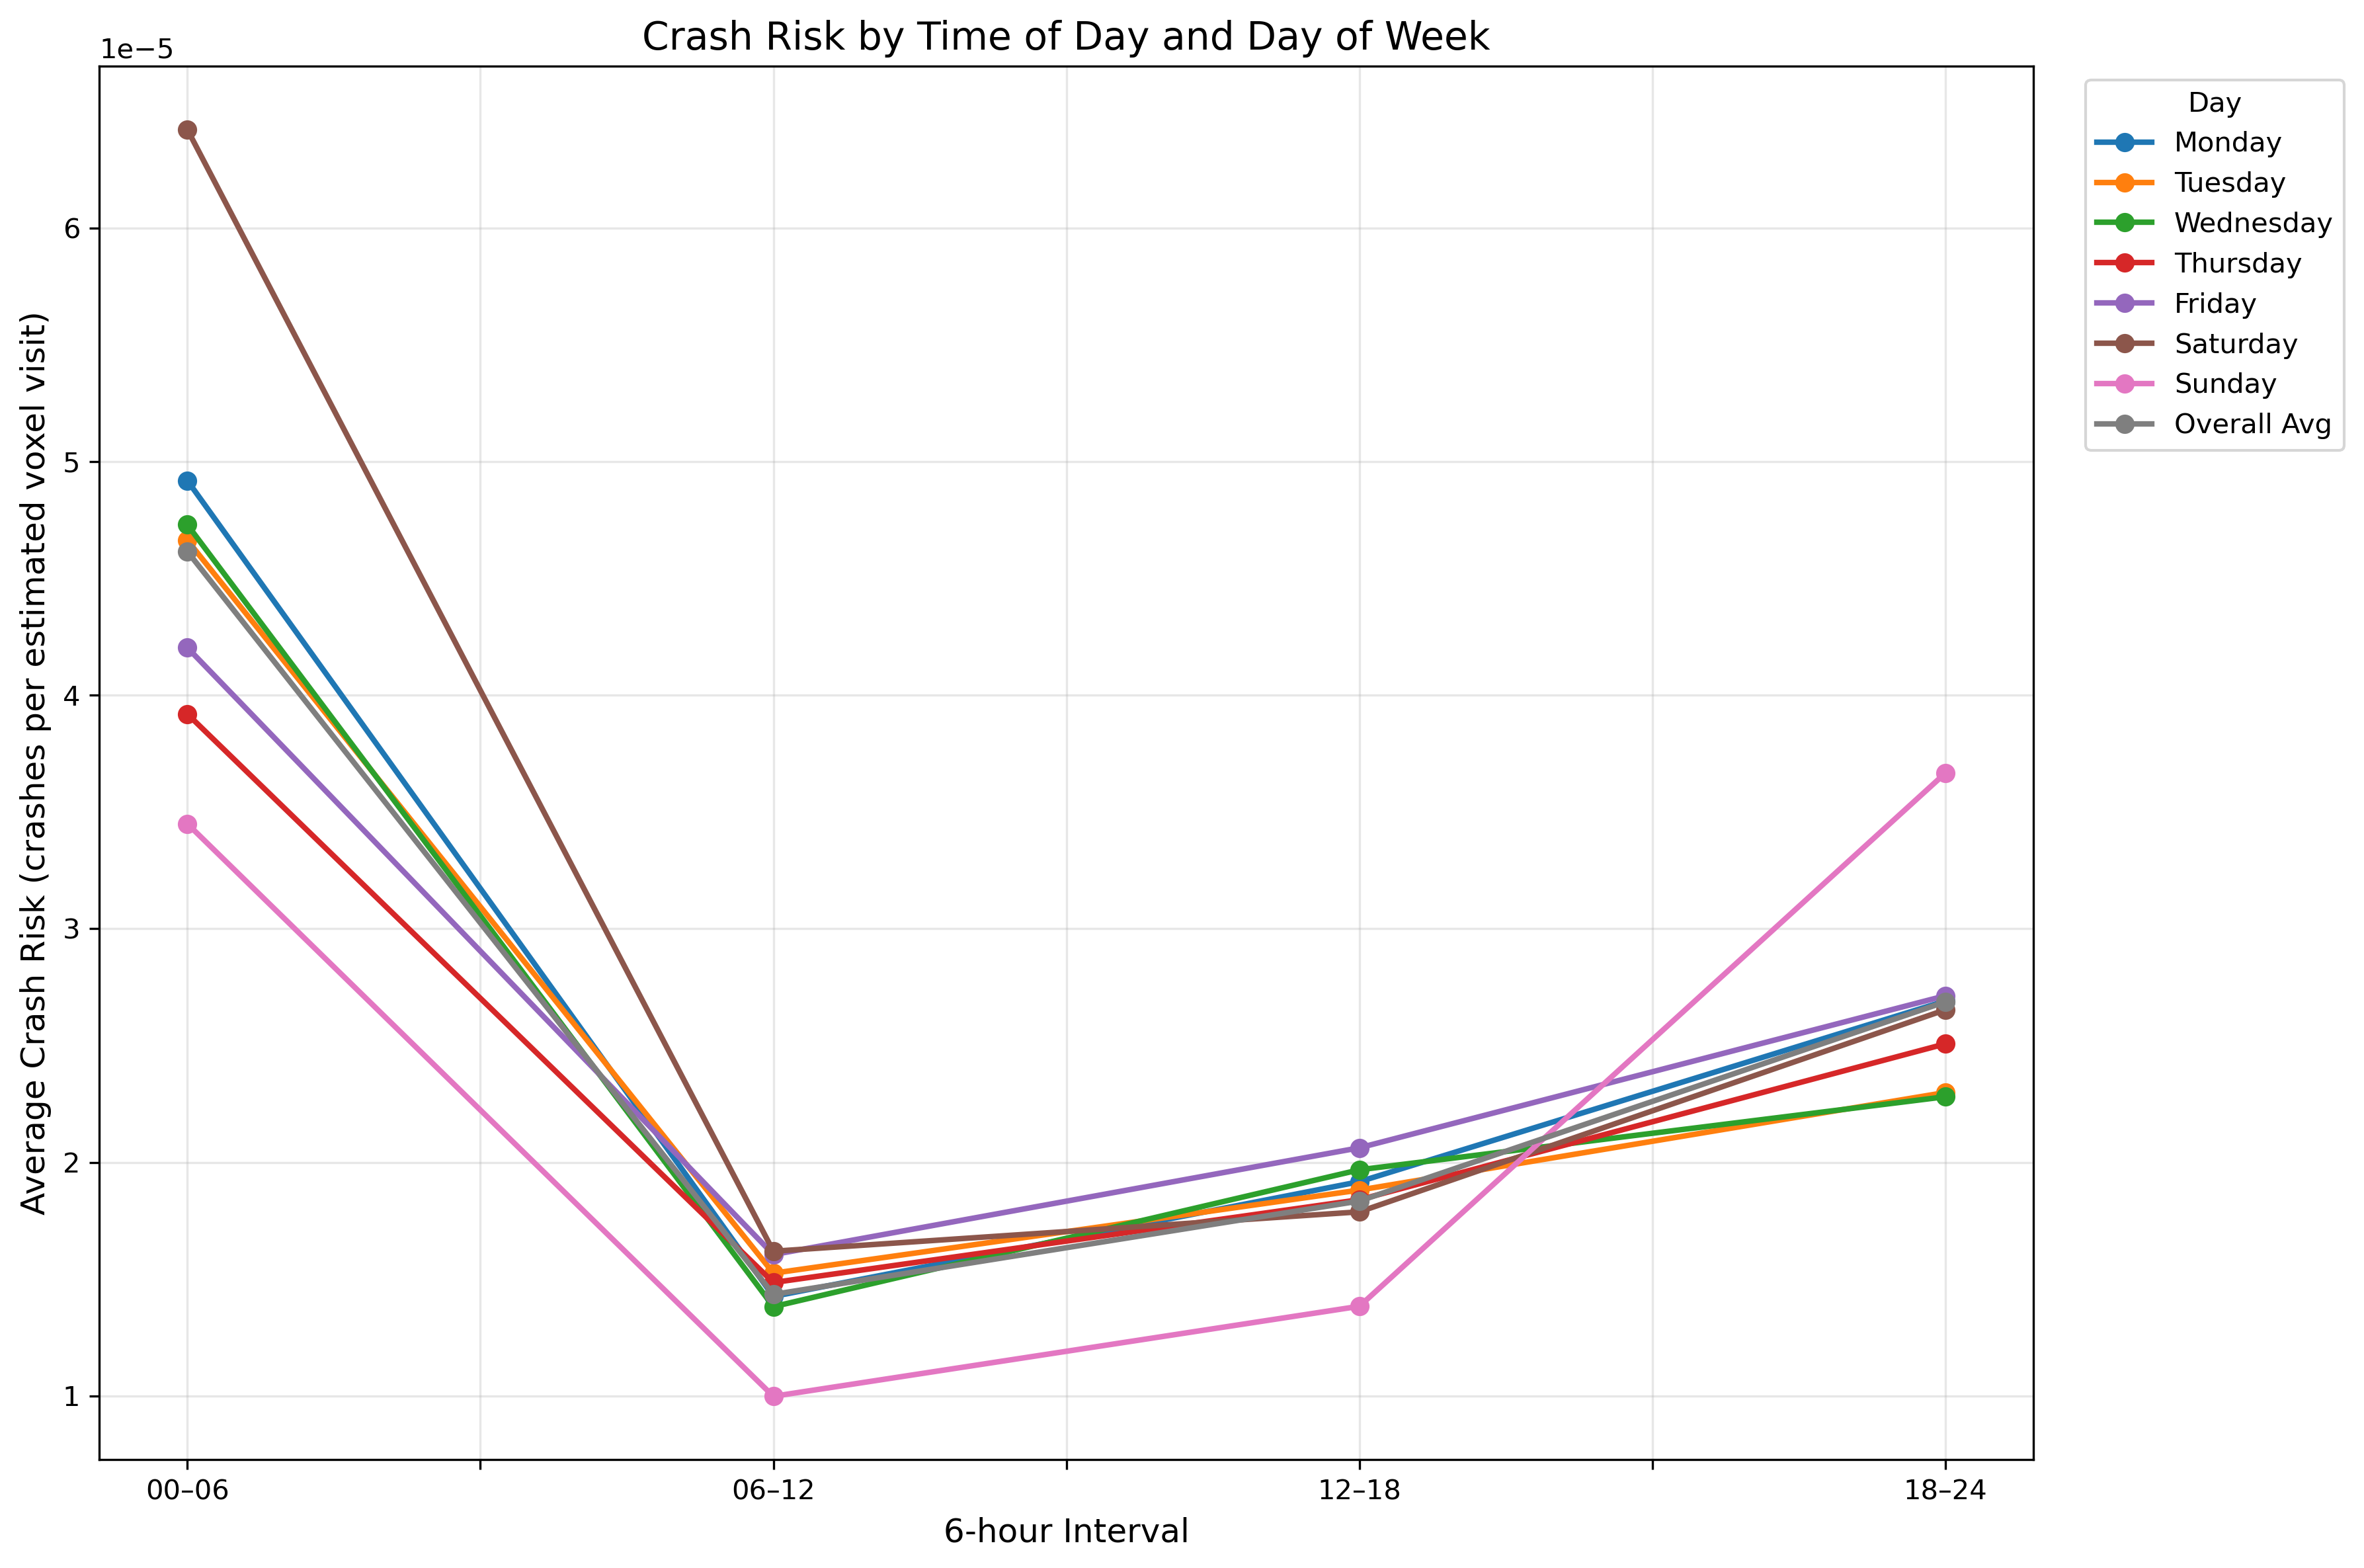
\includegraphics[width=0.9\textwidth]{../results/cellx800m_celly800m_cellt6h/plots/crash_risk_by_day_and_time_800.0m_800.0m_6.0h.png}
                \caption{Risk varies by day and time}
            \end{figure}
        \end{column}
        
        \begin{column}{0.43\textwidth}
            \begin{figure}
                \centering
                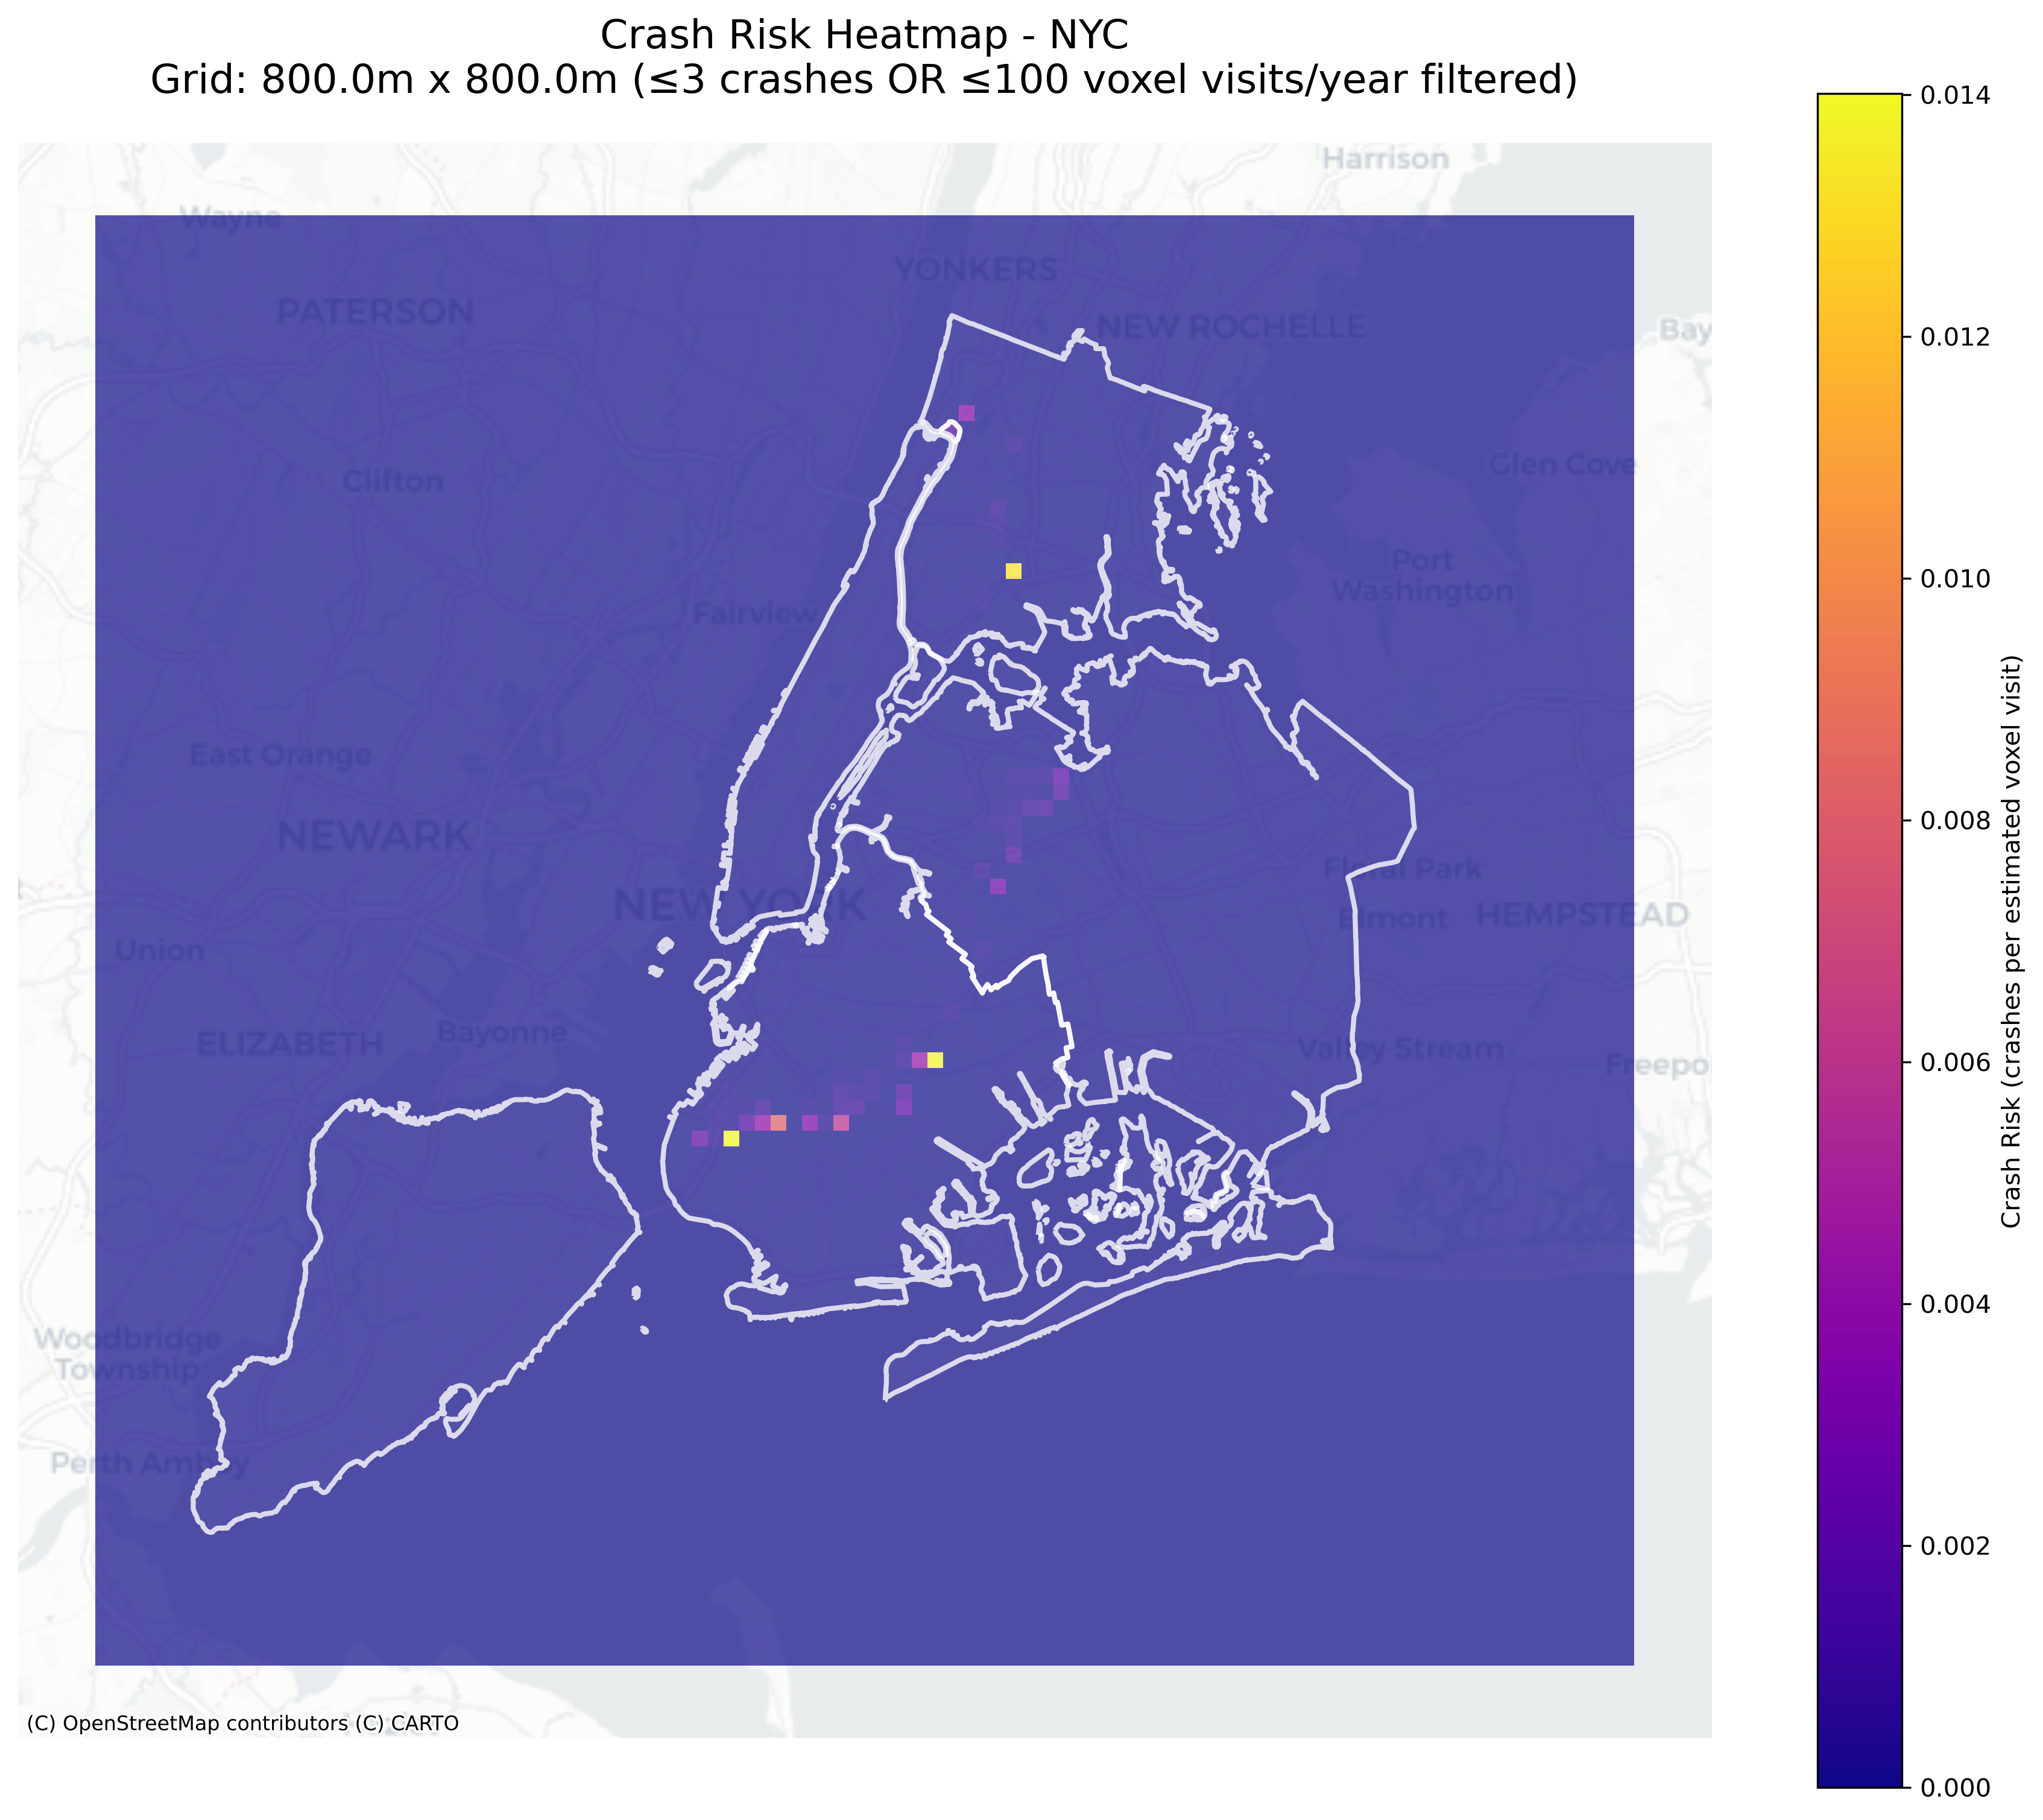
\includegraphics[width=0.9\textwidth]{../results/cellx800m_celly800m_cellt6h/plots/spatial_risk_heatmap_800.0m_800.0m_6.0h_filtered.png}
                \caption{Risk varies by location}
            \end{figure}
        \end{column}
    \end{columns}
    
    \vspace{0.3cm}
    \centering{\textbf{High spatial and temporal variability in crash risk}}
\end{frame}

%%%%%%%%%%%%%%%%%%%%%%%%%%%%%%%%%%%%%%%%%%%%%%%%%%%%%%%%%%%%%%%%%%%%%%%%%%%%%%%%
% Slide 5: Interacting effects and model challenges
%%%%%%%%%%%%%%%%%%%%%%%%%%%%%%%%%%%%%%%%%%%%%%%%%%%%%%%%%%%%%%%%%%%%%%%%%%%%%%%%

\begin{frame}{Complex Interacting Effects}
    \vspace{0.2cm}
    \begin{columns}
        \begin{column}{0.6\textwidth}
            \begin{figure}
                \centering
                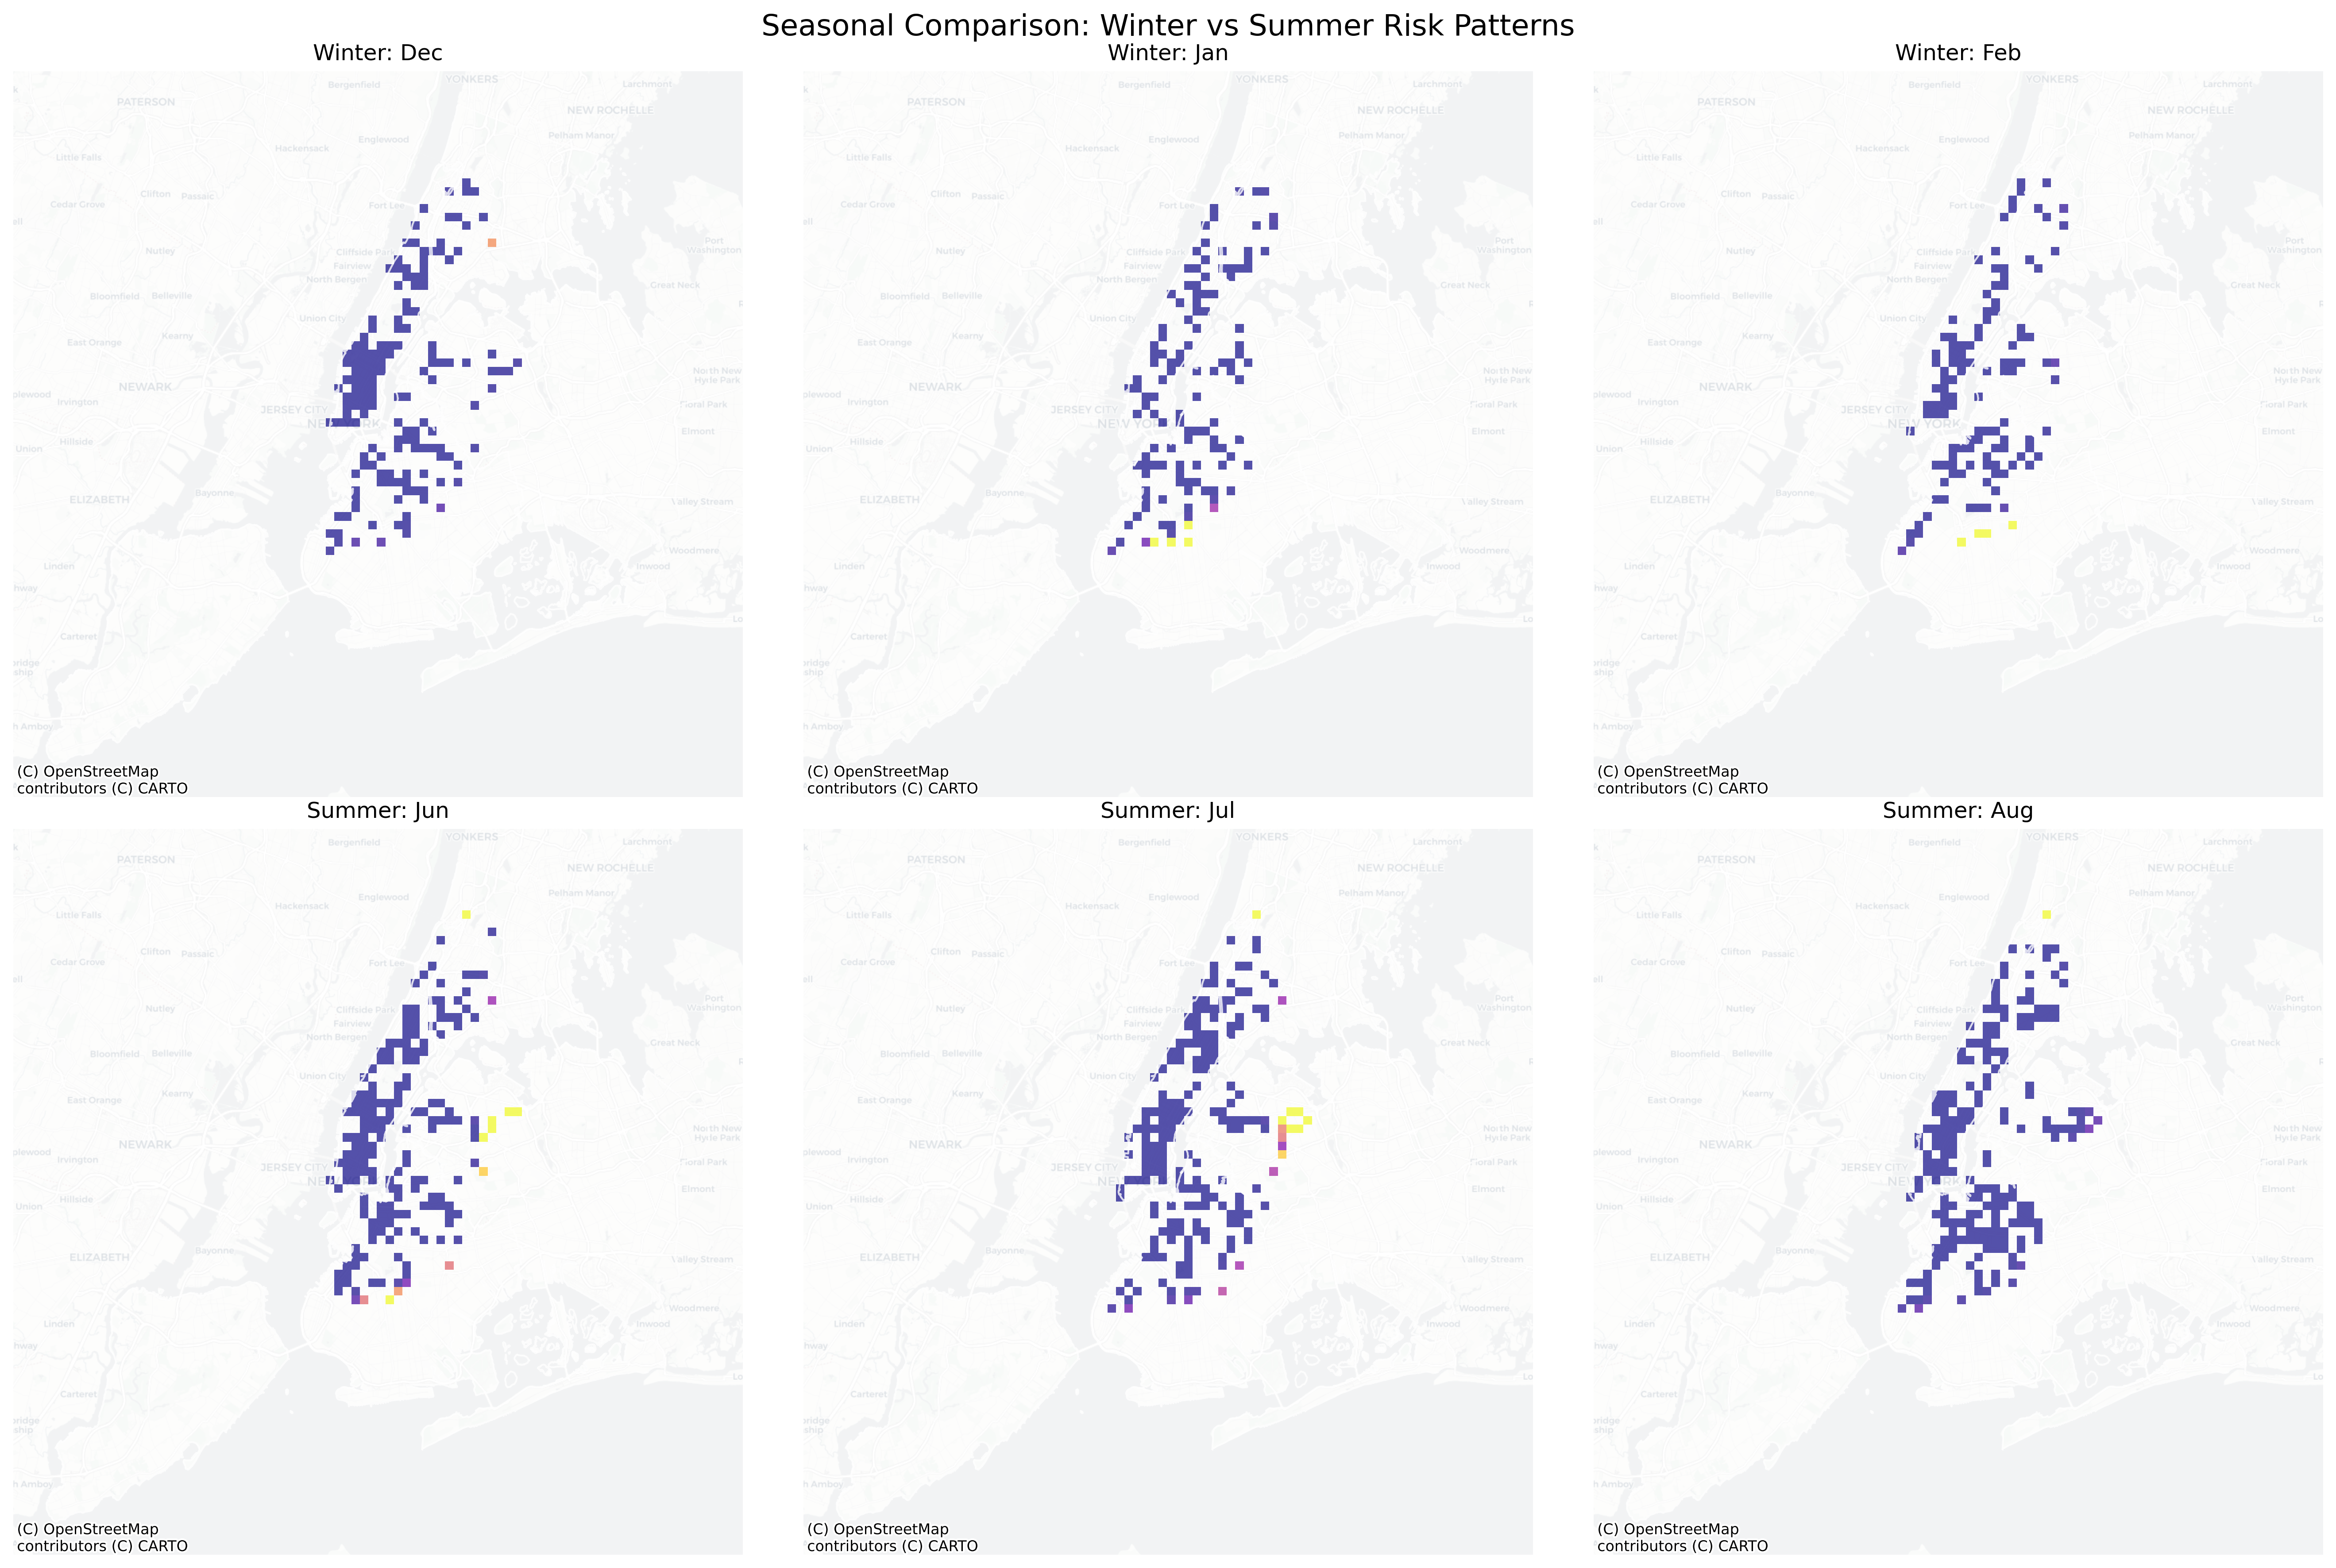
\includegraphics[width=\textwidth]{../results/cellx800m_celly800m_cellt6h/plots/seasonal_risk_comparison_800.0m_800.0m_6.0h.png}
                \caption{Seasonal risk patterns differ spatially}
            \end{figure}
        \end{column}

        \begin{column}{0.4\textwidth}
            \textbf{Problem:} Despite rough rasterization \\
            - spatial clusters are not homogeneous and inconsistent across time \textbf{and} \\
            - crash cases per voxel approach outlier territory.
        \end{column}
    \end{columns}
\end{frame}

%%%%%%%%%%%%%%%%%%%%%%%%%%%%%%%%%%%%%%%%%%%%%%%%%%%%%%%%%%%%%%%%%%%%%%%%%%%%%%%%
% Slide 6: Current Best Solution
%%%%%%%%%%%%%%%%%%%%%%%%%%%%%%%%%%%%%%%%%%%%%%%%%%%%%%%%%%%%%%%%%%%%%%%%%%%%%%%%
\begin{frame}{Current Best Solution: Simple, Digestible Rules}
    \vspace{0.3cm}
    \textbf{Honest assessment:} With current data alone, we cannot reliably identify specific danger zones. Instead, we should focus on easy rule.\\
    \vspace{0.3cm}
    \begin{itemize}
        \item \textbf{Time-based warnings:}
        \begin{itemize}
            \item Be extra careful during night hours and weekends
            \item Peak risk periods: Friday-Sunday evenings
        \end{itemize}
        
        \item \textbf{Location-based guidance:}
        \begin{itemize}
            \item Exercise caution in areas with low bike traffic
            \item Increased vigilance near highways and major intersections
            \item Avoid isolated routes during off-peak hours
        \end{itemize}
    \end{itemize}
    
    \vspace{0.4cm}
    \textbf{Future direction:} Predict dangerous areas ahead of time by integrating additional data sources (weather, traffic, events) and conduct careful re-analysis.
\end{frame}


%%%%%%%%%%%%%%%%%%%%%%%%%%%%%%%%%%%%%%%%%%%%%%%%%%%%%%%%%%%%%%%%%%%%%%%%%%%%%%%%
% Slide 7: Methods
%%%%%%%%%%%%%%%%%%%%%%%%%%%%%%%%%%%%%%%%%%%%%%%%%%%%%%%%%%%%%%%%%%%%%%%%%%%%%%%%
\begin{frame}{Implementation Details}
    For full details on data processing and analysis methods, please consult the documented source code:
    \begin{itemize}
        \item \texttt{src/apps/rasterize\_data.py}
        \item \texttt{src/utils.py}
        \item \texttt{src/jupyter/vis\_results.ipynb}
    \end{itemize}
\end{frame}

\end{document}